The peak detection script found the $^{241}$Am photopeak in channel 208 and the $^{137}$Cs photopeak in channel 2354. The documented energies for these photopeaks are 59.541 keV  and 661.657 keV, respectively. The identified photopeaks of $^{241}$Am and $^{137}$Cs are depicted in Figure \ref{fig:Peaks}.

\begin{figure}[H]
\centering
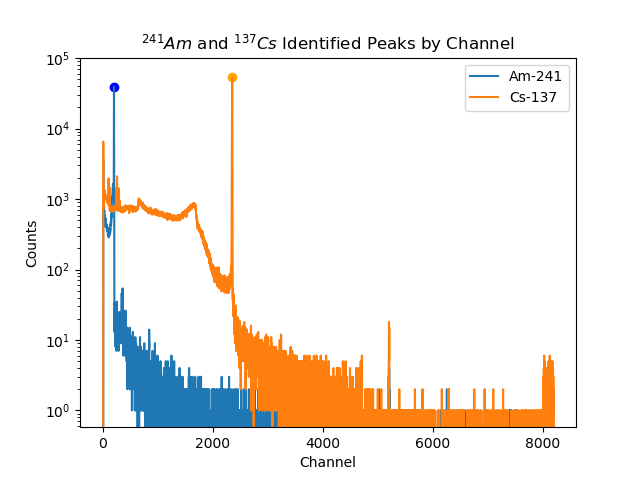
\includegraphics[scale=0.8]{images/Peaks.png}
\caption{Photopeaks of $^{241}$Am and $^{137}$Cs}
\label{fig:Peaks}
\end{figure}

The polyfit function found the linear relationship between channel and energy to be
\begin{align}
E_{calib} = 0.2805759552656106\cdot C + 1.1812013047530752 \label{eq:1}
\end{align}
where $E_{calib}$ is energy in keV and $C$ is channel number. Figure \ref{fig:Fit} depicts this linear calibration.

\begin{figure}[H]
\centering
\includegraphics[scale=0.8]{images/LinearFit.png}
\caption{Linear Fit of Channel to Energy}
\label{fig:Fit}
\end{figure}

The peak detection script found the $^{133}$Ba photopeaks in channels 13, 105, 284, 981, 1075, 1265, and 1364. However, the first two channels could be excluded from the data set because they are indicative of low energy noise and the 31 keV X-ray emitted by $^{133}$Ba. Figure \ref{fig:BaPeaks} depicts the photopeaks found in $^{133}$Ba.

\begin{figure}[H]
\centering
\includegraphics[scale=0.8]{images/BaPeaks.png}
\caption{$^{133}$Ba Photopeaks}
\label{fig:BaPeaks}
\end{figure}

The photopeaks for $^{133}$Ba were calculated using Equation \ref{eq:1}. Figure \ref{fig:BaSpecCal} depict the calibrated $^{133}$Ba spectrum and Table \ref{tab:Comp} shows a comparison of the calibrated and known peak energies for $^{133}$Ba.

\begin{figure}[H]
\centering
\includegraphics[scale=0.8]{images/BaSpecCal.png}
\caption{$^{133}$Ba Photopeaks}
\label{fig:BaSpecCal}
\end{figure}

\begin{table}[H]
\centering
\caption{Comparison of Photopeaks for $^{133}$Ba}
\label{tab:Comp}
\begin{tabular}{@{}ll@{}}
\toprule
Expected (keV) & Calibrated (keV) \\ \midrule
80.9979 & 80.86477260 \\
276.3989 & 276.42621342 \\
302.8508 & 302.80035322 \\
356.0129 & 356.10978472 \\
383.8485 & 383.88680429 \\ \bottomrule
\end{tabular}
\end{table}

The approximation error between calibrated and known energy values were quantified by Equations \ref{eq:2}, \ref{eq:3}, and \ref{eq:4}.
\begin{align}
\epsilon =\left | E_{calib}-E_{known} \right | \label{eq:2}
\end{align}
\begin{align}
\eta = \frac{\left | E_{calib}-E_{known} \right |}{E_{known}} \label{eq:3}
\end{align}
\begin{align}
\delta = \frac{\left | E_{calib}-E_{known} \right |}{E_{known}}\cdot 100 \label{eq:4}
\end{align}

\begin{table}[H]
\centering
\caption{Approximation Error in Calibrated $^{133}$Ba Photopeaks}
\label{tab:error}
\begin{tabular}{@{}llll@{}}
\toprule
$\gamma$ Energy & Absolute Error $\epsilon$ & Relative Error $\eta$  & Percent Error $\delta$ (\%) \\ \midrule
80.9979               & 0.1331273998135174        & 0.0016435907574581241  & 0.1643590757458124          \\
276.3989              & 0.027313420317000237      & 9.881884593969163e-05  & 0.009881884593969163        \\
302.8508              & 0.05044678471557518       & 0.00016657306077968155 & 0.016657306077968153        \\
356.0129              & 0.09688471575043422       & 0.00027213821676246627 & 0.027213821676246627        \\
383.8485              & 0.038304287045889396      & 9.979011783526416e-05  & 0.009979011783526417        \\ \bottomrule
\end{tabular}
\end{table}
